% vim: set spelllang=fr foldmethod=marker:
\section{Quelques problématiques}

De par leurs ressources faibles, leur dispersion dans un environnement parfois hostile, leurs communications sans fil, et les différentes missions qui leur sont confiées, les \rcsfs introduisent une multitude de problématiques que l'on ne retrouve pas ou peu dans d'autres types de réseaux.
Nous introduisons ici celles qui sont indispensables à la compréhension des travaux de cette thèse.

    \subsection{Gestion des ressources et performances}


Power conservation and security enhancement in WSNs - a priority based approach (2014 Sivakumar Amirthavalli Senthil)

K. Piotrowski, P. Langendoerfer, and S. Peter. How Public Key Cryptography Influences Wireless Sensor Node Lifetime. In Proc. of the 4th ACM SASN, 2006.
PLP06

Y. Law, J. Doumen, and P. Hartel. Survey and benchmark of block ciphers for wireless sensor networks. Technical Report TR-CTIT-04-07, Centre for Telematics and Information Technology, University of Twente, The Nether- lands, 2004.


In addition, WSNs have following specific objects:
- Scalability: supporting a great number of nodes
- Efficiency: storage, processing and communication limitations on sensor nodes must be
considered
(2008 Li Gong)


L'une des possibilités permettant de réduire la consommation en énergie est l'utilisation d'un réseau \index{clusterisation!clusterisation hiérarchique} hiérarchiquement clusterisé.

    \subsection{Partition hiérarchique des nœuds du réseau}%
    \label{st:subsec:partition}

        \subsubsection{Partition du réseau}
«~Clusteriser~» un ensemble d'éléments revient à le diviser en sous-ensembles appelés \textit{clusters}.
Dans le cas des \rcsfs, cette partition permet d'obtenir un routage efficace des paquets, en adoptant la configuration suivante:
\begin{enumerate}
    \item tous les nœuds réunis au sein d'un même cluster sont capables de communiquer directement entre eux (\textit{one-hop transmission});
    \item lors de la partition, un unique nœud par cluster est désigné «~chef~» du cluster.
        Il est choisi, de façon déterministe ou bien aléatoire selon l'algorithme employé, parmi les nœuds «~normaux~» du cluster.
        Ce «~chef~» est appelé \ch (\CH);\nomenclature{CH}{\textit{Cluster Head}}
    \item lorsqu'un capteur quelconque d'un cluster souhaite faire parvenir des informations à un nœud d'un autre cluster\footnote{Pour une grande partie des applications, les communications entre nœuds de différents clusters, hors \chs, ne se produisent pas. La totalité du trafic «~utile~», acheminant des données, est généralement à destination de la \sdb.}, ou bien à la \sdb, il envoie ses paquets de données au \ch de son cluster ;
    \item le \ch transmet alors les paquets de données, soit directement à la cible s'il s'agit de la \sdb et qu'il peut l'atteindre, soit en passant par d'autres \chs (\textit{multi-hops transmission}), jusqu'à atteindre le destinataire.
\end{enumerate}
Le schéma d'un réseau clusterisé est présenté en \figref{st:fig:wsn}.
\begin{figure}
    \centering
    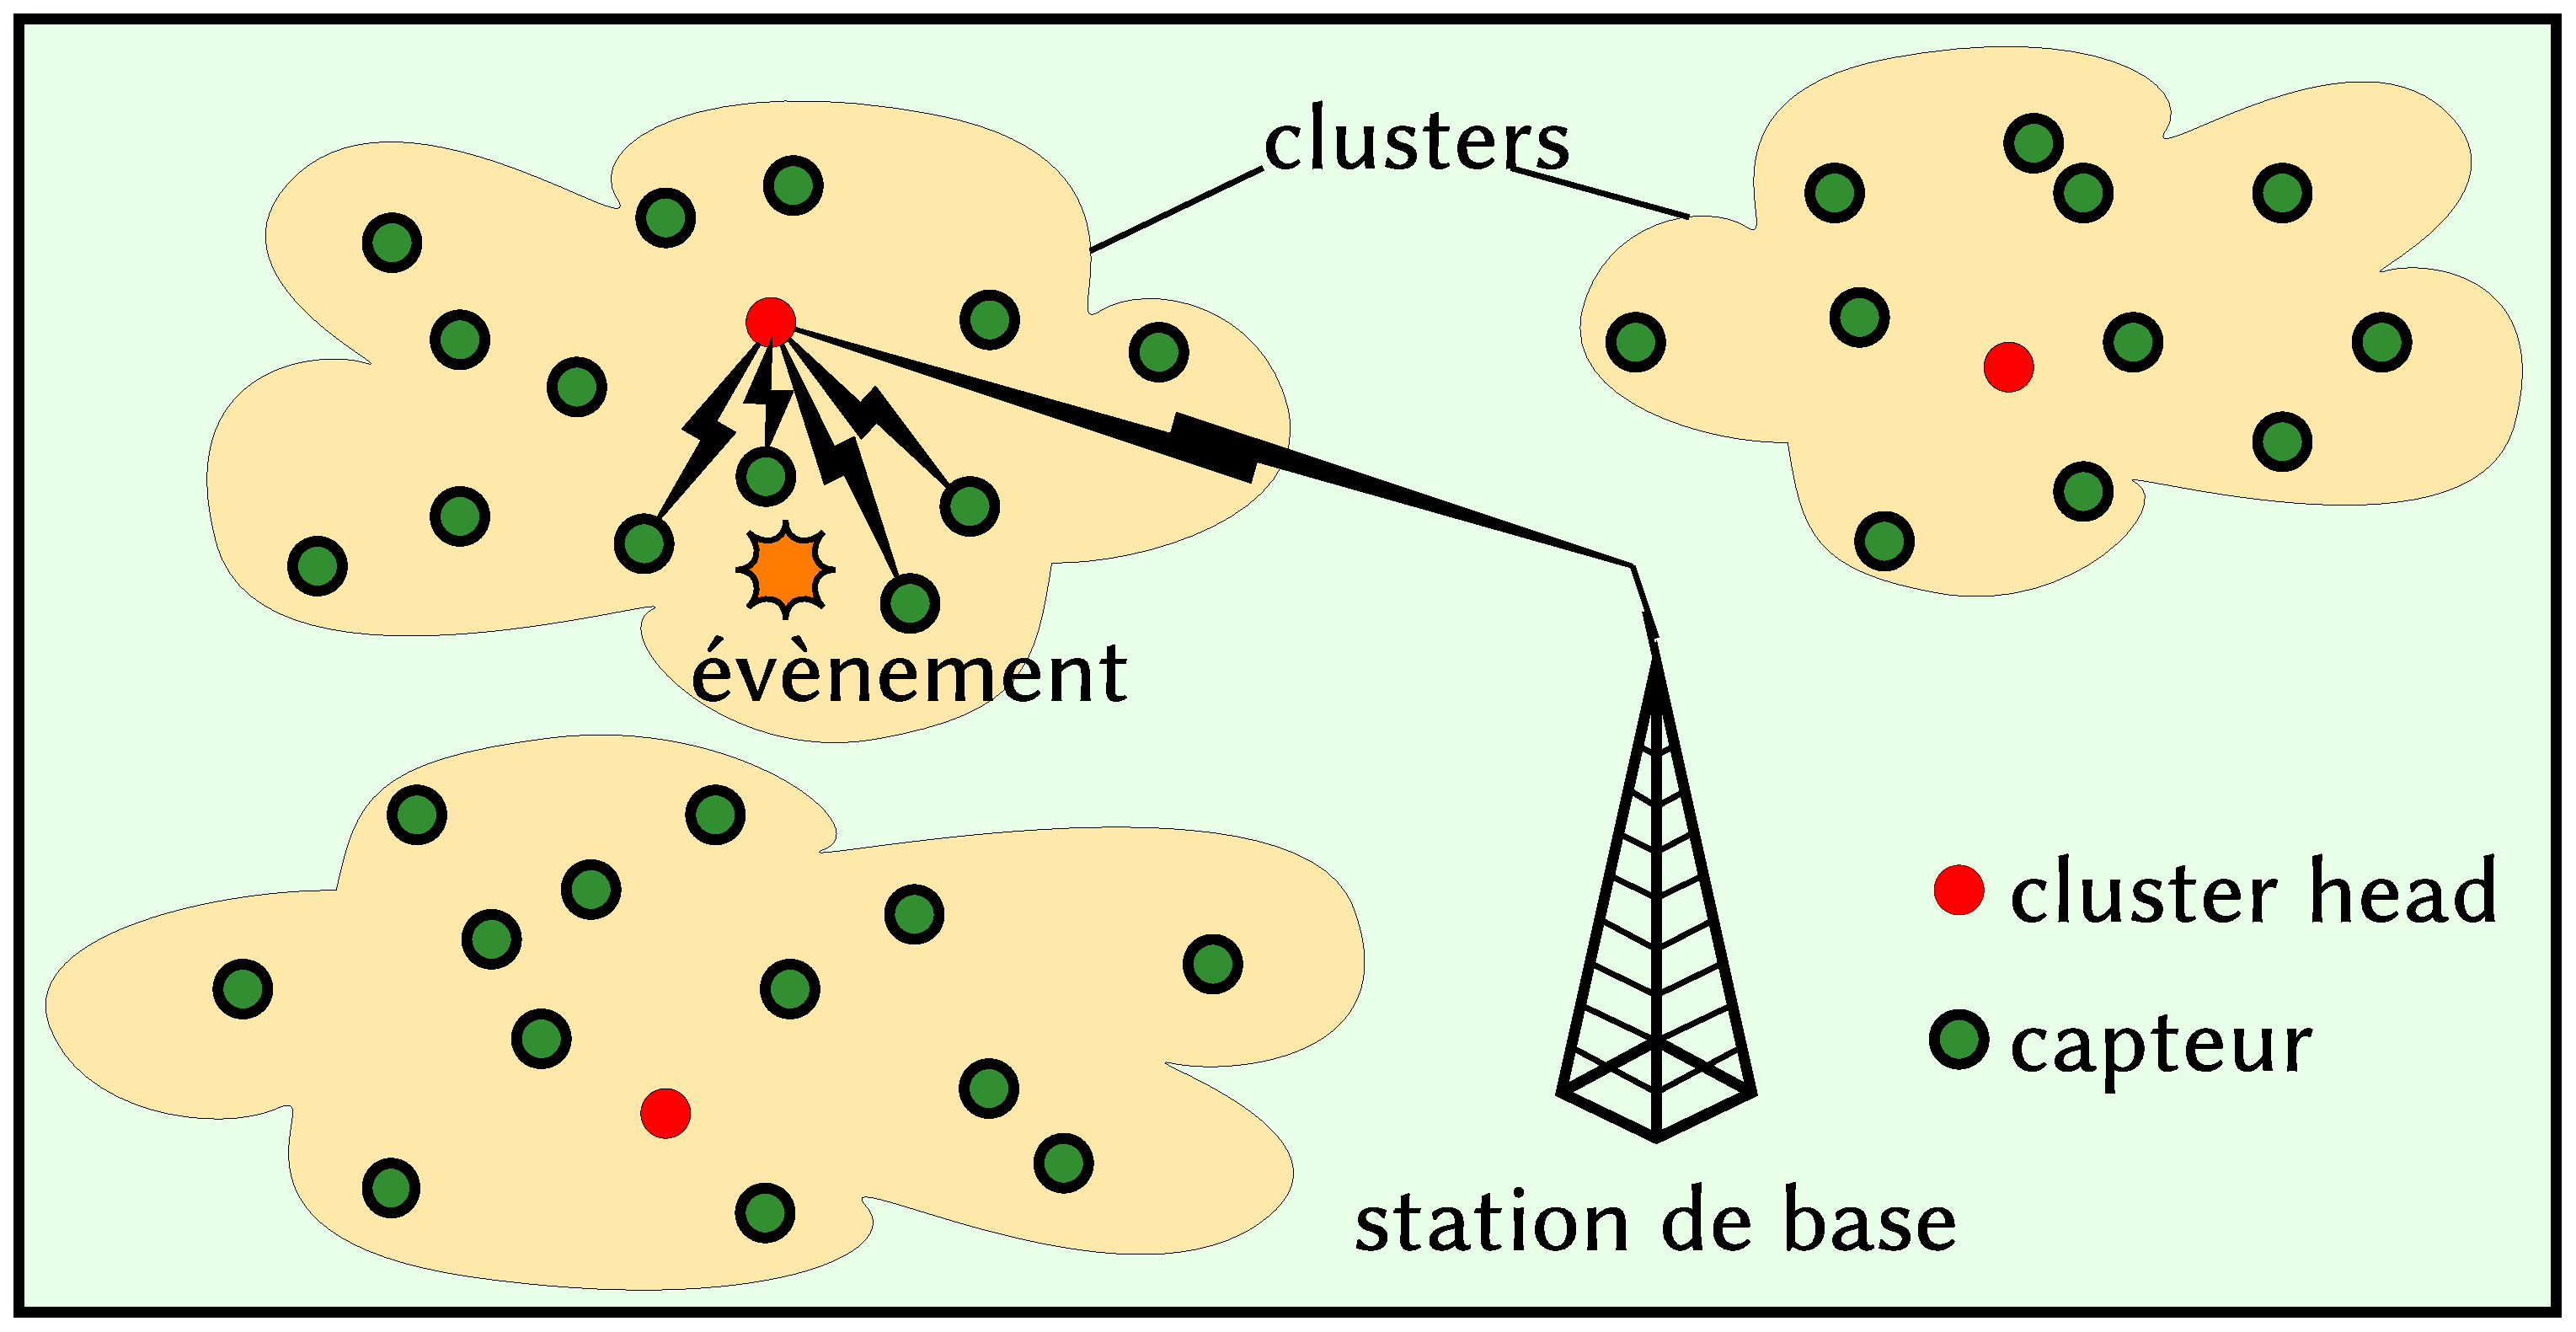
\includegraphics[width=0.8\linewidth]{\chapterfig/WSN.eps}
    \caption{Schéma d'un \rc clusterisé}\label{st:fig:wsn}
\end{figure}
L'appel à un algorithme de « \idx{clusterisation} » a pour effet de limiter les émissions à «~longue portée~» (relativement aux communications intra-clusters) aux \chs seulement.
Hors les communications sur de plus grandes distances se traduisent par une plus grande consommation en énergie (puisqu'une plus grande puissance d'émission est nécessaire).
Les capteurs «~normaux~» (non \chs) n'ont pas à atteindre directement des nœuds situés en dehors de leur cluster; ils économisent d'autant en énergie.
De plus, dans la limite de leurs capacités, les \chs sont généralement amenés à réaliser des opérations d'\idx{agrégation} voire parfois de \idx{compression} sur les paquets qu'ils reçoivent, afin de limiter encore les transmissions couteuses.

De nombreux algorithmes de \idx{clusterisation} de données existent.
Plusieurs d'entre eux sont même spécifiquement adaptés aux \rcsfs.
Parmi les plus fréquemment utilisés, on trouve des algorithmes comme \leach~\cite{HCB00} ou \heed~\cite{YF04}.
D'autres sont moins connus, comme \ffuca~\cite{FL11}, qui repose sur l'exploitation de propriétés ultramétriques dans le réseau.
\nomenclature{LEACH}{\textit{Low-Energy Adaptive Clustering Hierarchy}}
\nomenclature{HEED}{\textit{Hybrid, Energy-Efficient Distributed clustering}}
\nomenclature{FFUCA}{\textit{Fast and Flexible Unsupervised Clustering Algorithm }}

        \subsubsection{Clusterisation hiérarchique\index{clusterisation!clusterisation hiérarchique}}
Une fois le \rc divisé en clusters, rien n'empêche de considérer les clusters un à un et de leur appliquer à nouveau un algorithme de \idx{clusterisation}, de façon à établir des sous-ensembles dans chaque cluster.
Et ainsi de suite, de façon récursive, jusqu'à atteindre le degré de hiérarchie désiré.
L'intérêt de cette méthode est de créer une partition hiérarchique dans le réseau, permettant un meilleur contrôle des sous-ensembles de capteurs.
Par ailleurs, les clusters situés tout en bas dans la hiérarchie constituée seront de petite taille.
Les communications intra-clusters seront donc peu consommatrices en énergie.

Pour pouvoir distinguer plus facilement le niveau de hiérarchie auquel nous nous plaçons, nous désignerons par la suite sous le terme \textit{$k$-cluster} ($0 \leq k \leq$~nombre de capteurs) un sous-ensemble obtenu après $k$ applications de l'algorithme de \idx{clusterisation}.
En suivant cette convention, l'unique $0$-cluster est alors le réseau tout entier.
Lorsque nous parlons simplement de \textit{clusters}, il faudra comprendre \textit{$1$-clusters}; autrement dit, des clusters issus d'une partition simple, sans degré supplémentaire de hiérarchie.

De même, on désignera par \textit{$k$-\ch} (ou bien par \textit{$k$-CH}) les \chs de chacun des $k$-clusters du réseau.
Le rôle de $0$-cluster pourra alors être attribué à la \sdb.
Chaque \textit{$k$-CH} reçoit des données (provenant soit de nœuds normaux si $k$ est le dernier degré de la hiérarchie constituée, soit de \textit{$k+1$-CH}), les agrège et les transmet au \textit{$k-1$-CH} auquel il est rattaché.

        \subsubsection{Exemple: fonctionnement de l'algorithme \leach}%
        \label{st:subsubsec:leach}
L'un des algorithmes de \idx{clusterisation} les plus simples et les plus couramment employés dans les \rcsfs est l'algorithme \leach (\textit{Low Energy Adaptive Clustering Hierarchy with deterministic \ch selection}).
Il s'agit d'un algorithme dynamique (il effectue de nouvelles clusterisations\index{clusterisation} du réseau régulièrement dans le temps) qui, par la formation de clusters, met en place une solution de routage des paquets dans le réseau.

Voici le fonctionnement détaillé de cet algorithme.
Soit $P$ le pourcentage moyen de clusters que nous désirons obtenir dans le réseau à un instant quelconque $t$.
\leach est découpé (dans la durée) en cycles, chacun constitué de $\frac{1}{P}$~rondes.
Chaque ronde $r$  est organisée de la façon suivante:
\begin{enumerate}
    \item Chaque nœud du réseau à partitionner calcule une valeur de seuil $S(i)$:
        \[
            S(i) = \left\{
            \begin{array}{cl}
                \displaystyle \frac{P}{1-P\cdot\left(r\mbox{ mod }\frac{1}{P}\right)} & \mbox{si }i\mbox{ n'a pas encore été \CH}\\
                                                                                    0 & \mbox{si }i\mbox{ a déjà été \CH}
            \end{array}
            \right.
        \]
        Chaque nœud choisit un nombre pseudo-aléatoire $0 \le x_{i}\le 1$.
        Si $x_{i} \le S(i)$, alors $i$ s'auto-désigne comme \CH pour la ronde en cours.
        Il est à noter que le calcul de $S(i)$ est réalisé de telle façon que chaque nœud devienne \ch une fois et une fois seulement au cours de chaque cycle de $\frac{1}{P}$~rondes: le taux de probabilité d'auto-désignation $S(i)$ est égal à $1$ lorsque la fin du cycle est atteinte (autrement dit, lorsque $r = \frac{1}{P}-1$).
    \item Les \chs auto-désignés informent leurs nœuds voisins de leur changement de statut à l'aide de messages en \textit{broadcast}.
        Tous ces messages sont envoyés en utilisant la même puissance de transmission (valeur fixe et prédéterminée lors de l'implémentation).
        Pour limiter les collisions, il est fait usage de la méthode \textit{Carrier Sense Multiple Access} (\csma) au niveau de la couche MAC.
    \item Les autres nœuds, qui ne se sont pas désignés en tant que \chs pour la ronde en cours, choisissent de se joindre au cluster du \CH dont ils perçoivent le signal avec l'intensité la plus élevée, \cad le \CH le plus proche en termes d'émissions électromagnétiques.
        Chaque nœud prévient le \ch qu'il décide de rejoindre en lui envoyant un message.
        La méthode \csma est là encore appliquée.
    \item Au vu des réponses reçues, chaque \ch calcule un «~ordre de transmission~» pour les nœuds qui l'ont rejoint.
        Il annonce alors à chacun de ces nœuds l'instant auquel le nœud doit lui transmettre ses données.
        Dans chaque cluster, les nœuds s'adresseront donc à leur \ch à tour de rôle, selon l'ordre déterminé par le \CH, ce qui revient à utiliser la méthode appelée \textit{Time Division Multiple Access} (\tdma).
    \item La phase de collecte des données peut débuter.
        Les \chs restent en écoute et reçoivent les données des autres capteurs de leur cluster.
        Les capteurs «~normaux~» effectuent leur mission (en général, ils réalisent des mesures sur leur environnement), et envoient leurs résultats au \ch lorsque c'est à leur tour de le faire.
        Lorsque ce n'est pas à leur tour de communiquer, ces nœuds mettent leur équipement radio en veille afin d'économiser leur énergie.
        Les collisions entre les transmissions des nœuds de différents clusters sont évitées grâce à la méthode appelée \textit{Code Division Multiple Access} (\cdma).
    \item Au fur et à mesure qu'ils reçoivent les données, les \chs agrègent\idx{agrégation}, et éventuellement compressent\idx{compression} ces dernières.
        Ils les envoient ensuite à la \sdb, soit au cours d'une unique transmission directe, soit en faisant relayer les paquets par d'autres \chs.
    \item Les étapes~5 et~6 sont répétées jusqu'à la fin de la ronde.
\end{enumerate}

Plusieurs remarques sont à énoncer.
Tout d'abord: pour un cluster donné, il est alors possible de réitérer l'application de l'algorithme \leach, afin de créer une nouvelle partition au sein même d'un cluster.
Et ainsi de suite par récursivité, jusqu'à obtenir le degré de hiérarchie\index{clusterisation!clusterisation hiérarchique} désiré dans le réseau.
Nous appellerons $k$-\leach cet algorithme appliqué de façon à créer $k$ degrés hiérarchiques.

Seconde remarque: il est possible d'étendre \leach pour prendre en compte l'énergie restante dont dispose chaque nœud lors de l'élection des \CH.
Cette énergie restante intervient alors en temps que paramètre supplémentaire lors du calcul de la valeur de seuil $S(i)$~\cite{HHT02}.

Troisième point: l'un des aspects importants de \leach est que lors de la première étape, chaque nœud choisi d'être, ou non, un \ch pour la ronde en cours.
Ce choix est basé uniquement sur la valeur de seuil calculée, et sur le nombre pseudo-aléatoire généré; à aucun moment un nœud ne fait intervenir dans sa décision le comportement de ses voisins.
En conséquence, le pourcentage $P$ de \chs désirés dans le réseau n'est qu'une valeur moyenne sur l'ensemble des rondes de chaque cycle.
Par ailleurs, la répartition géographique (au regard de la puissance de transmission nécessaire) idéale des \chs n'est en rien assuré.
Au contraire, il est même probable d'obtenir, pour certaines rondes, une concentration importante de \chs dans une zone restreinte du réseau, tandis que d'autres régions seront mal couvertes.
Il n'y a pas grand-chose à faire dans ce cas, sinon espérer que la prochaine ronde sera plus favorable.
Si toutefois un nœud ne parvient à capter les messages d'aucun \ch, il se déclare généralement lui-même \CH.

        \subsection{Sécurité, \idx{sureté} et \resilience}

%La sureté et la résilience des réseaux ne sont pas des problématiques de sécurité (car aucune attaque volontaire ne rentre en compte), mais il s'agit de problématiques assez proches de la disponibilité des réseaux.

        \subsubsection{Sécurité}
En raison de leurs faibles capacités, conjuguées aux domaines critiques dans lesquels ils interviennent parfois, les capteurs peuvent présenter des cibles de choix pour un attaquant.
Les algorithmes et mécanismes classiques utilisés en \idx{cryptographie} afin d'assurer la confidentialité ou l'authentification des données sont souvent très exigeants en ressources (en termes de calculs notamment, et donc de consommation énergétique).
Il a fallu adapter ces mécanismes aux capteurs.

D'autres attaques peuvent être menées, non plus pour intercepter des données, mais dans le but de perturber le bon fonctionnement du réseau.
Ce sont les attaques dites de \textit{\dds}.
Un attaquant, par le biais d'un nœud compromis par exemple, peut ainsi chercher à détourner des flux de données au sein du réseau, à empêcher des paquets de parvenir à destination (en les supprimant), à maximiser le débit du nœud compromis au détriment de celui des autres nœuds, à saturer le canal de transmission pour empêcher les nœuds légitimes de l'utiliser, ou encore à pousser les autres capteurs à l'épuisement de leurs réserves en énergie, \etc.
Les problématiques de sécurité dans les \rcs sont développées plus en détail dans le \chapref{ea}.

\todo{Corriger ici}
Notre but est ici de proposer, modéliser et tester une solution permettant de détecter, puis de réagir à une attaque de ce type, tout en assurant une consommation minimale en ressources pour les capteurs du réseau.

        \subsection{Déploiement autonome, \idx{mobilité}}
    scalabilité

    MANET, VANET
\nomenclature{MANET}{\textit{Mobile Ad hoc Networks}}
\nomenclature{VANET}{\textit{Vehicular Ad hoc Networks}}
